%%% SVN stuff
\svnid{$Id: SystemOverview.tex 128 2024-07-14 20:00:16Z KneadProject $}

The \ThisSystem is a game that users an play a game.

Figure~\ref{fig:SystemOverview} shows the high-level architecture for the \ThisSys system. 
\begin{figure}[htbp]
	\centering
	\ifpdf
			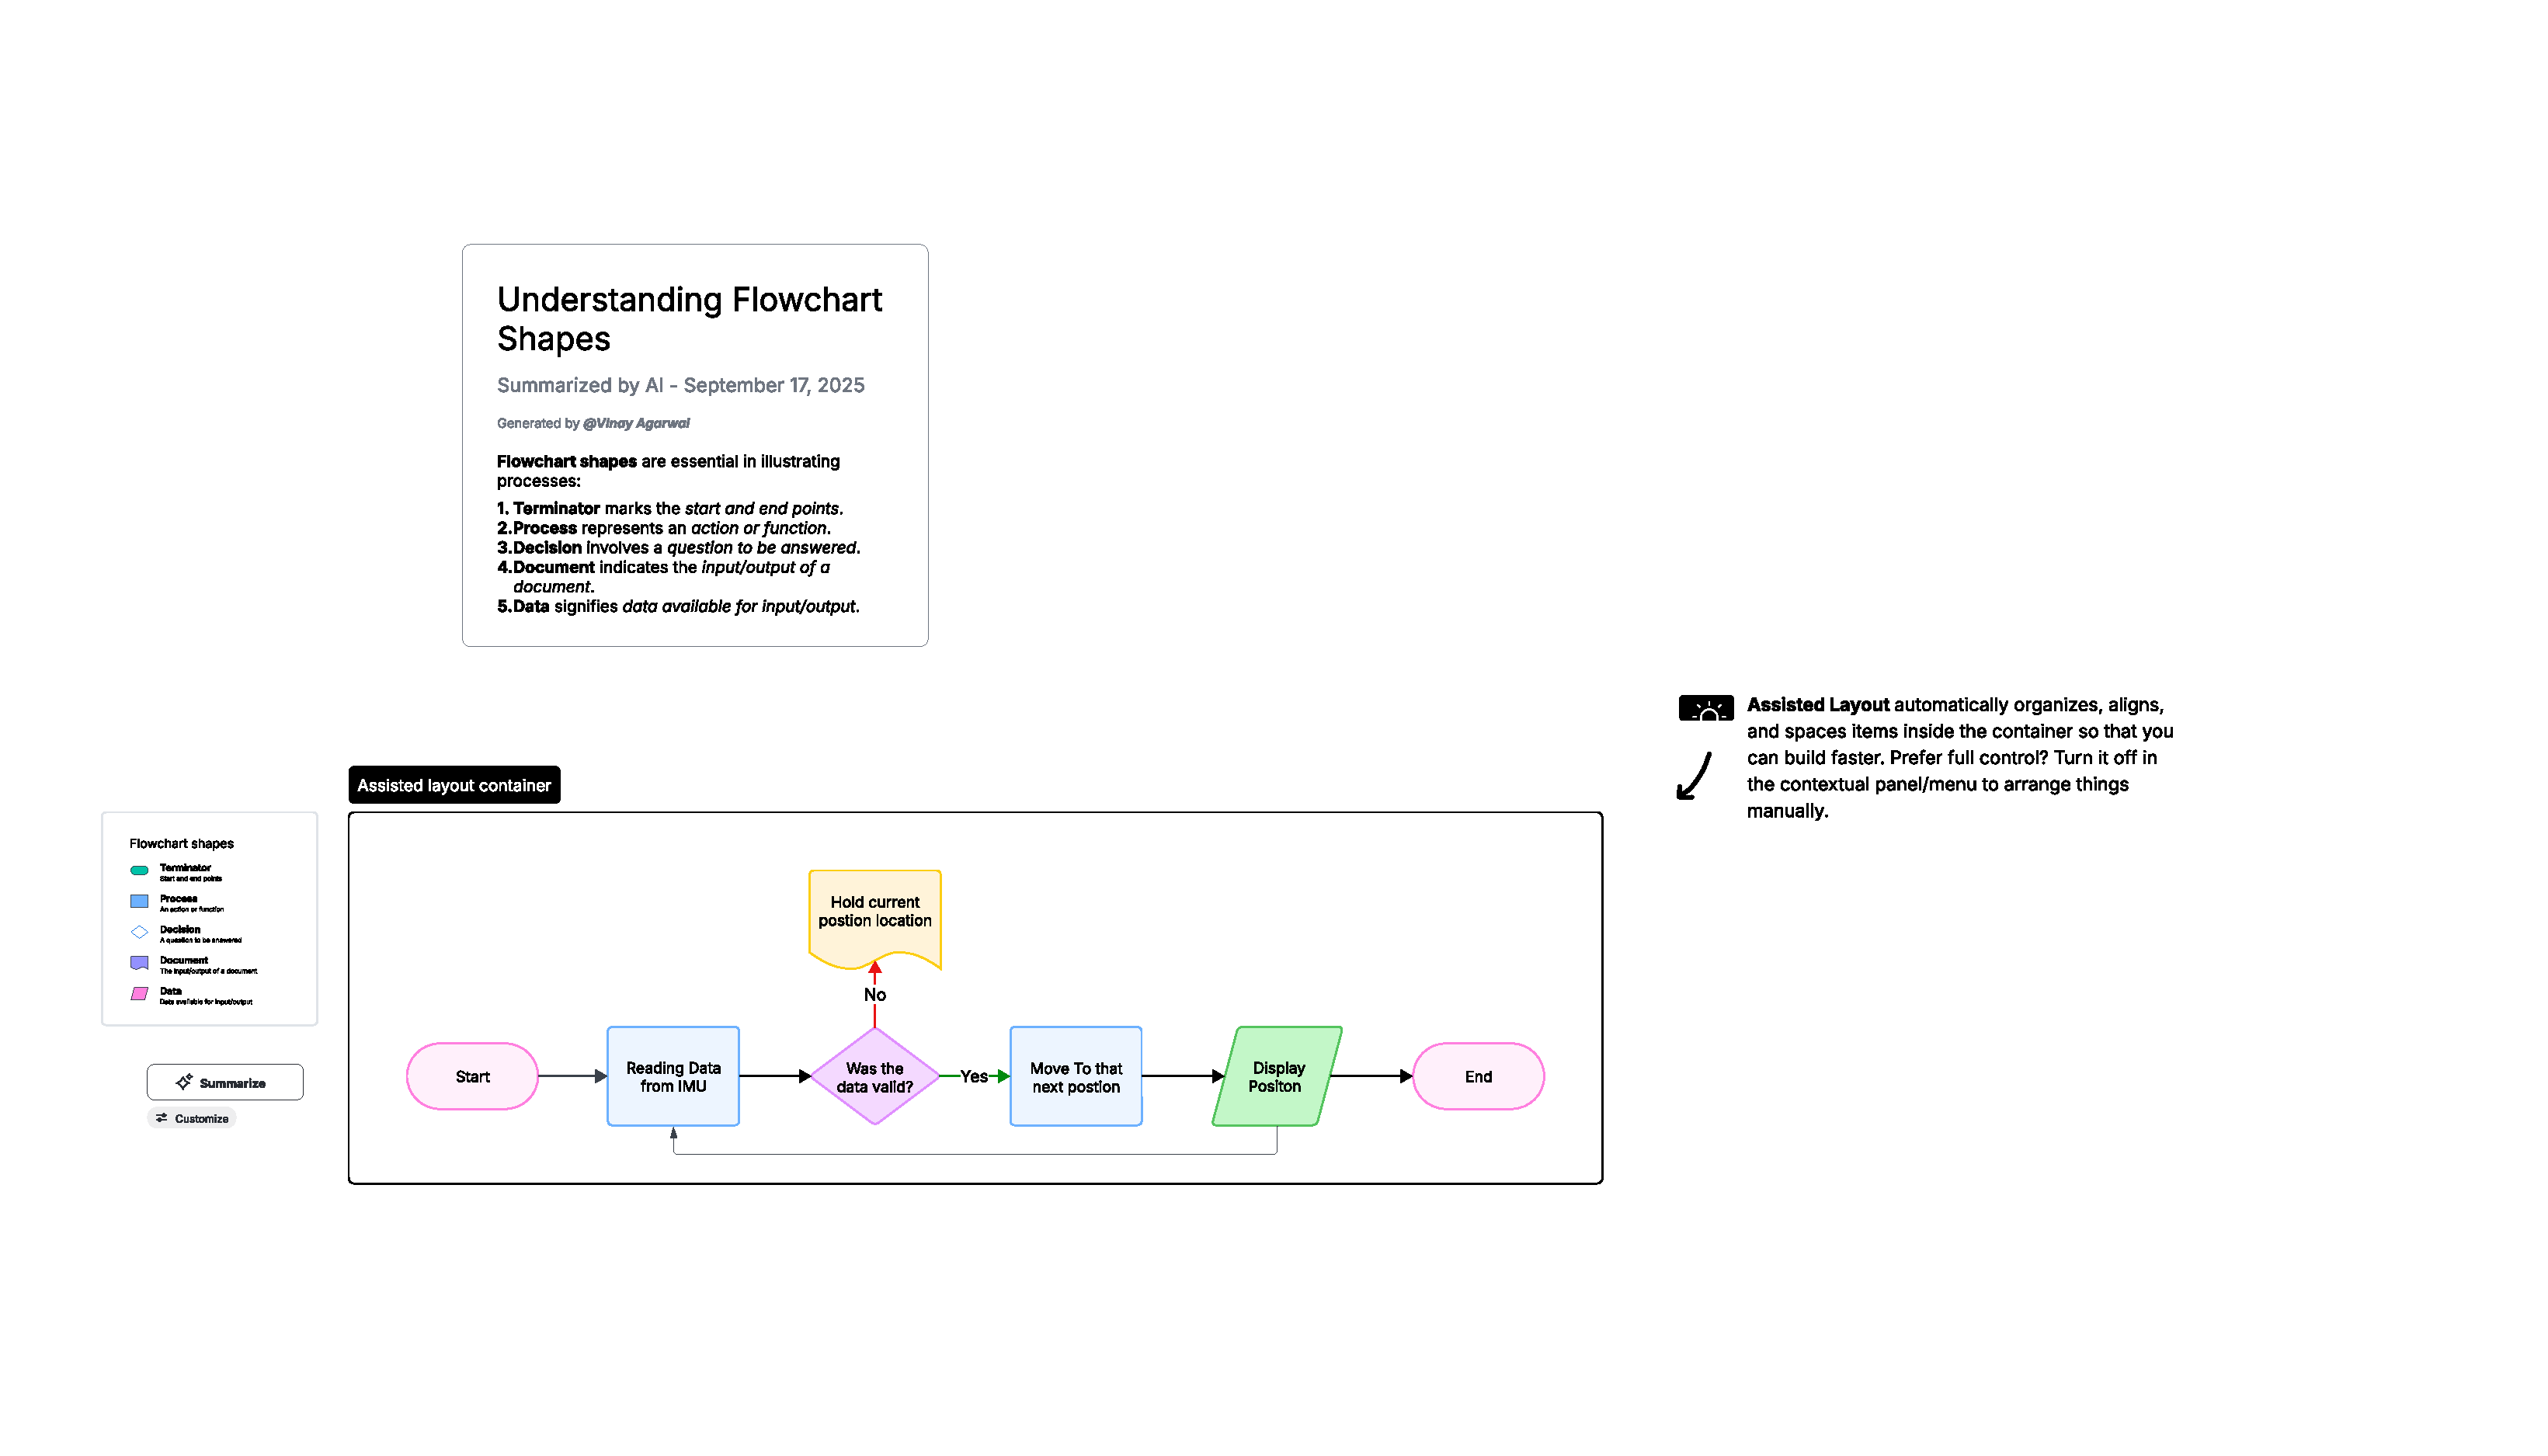
\includegraphics[width=6in]{../zProjectWideData/images/Diagram.pdf}
		\else
			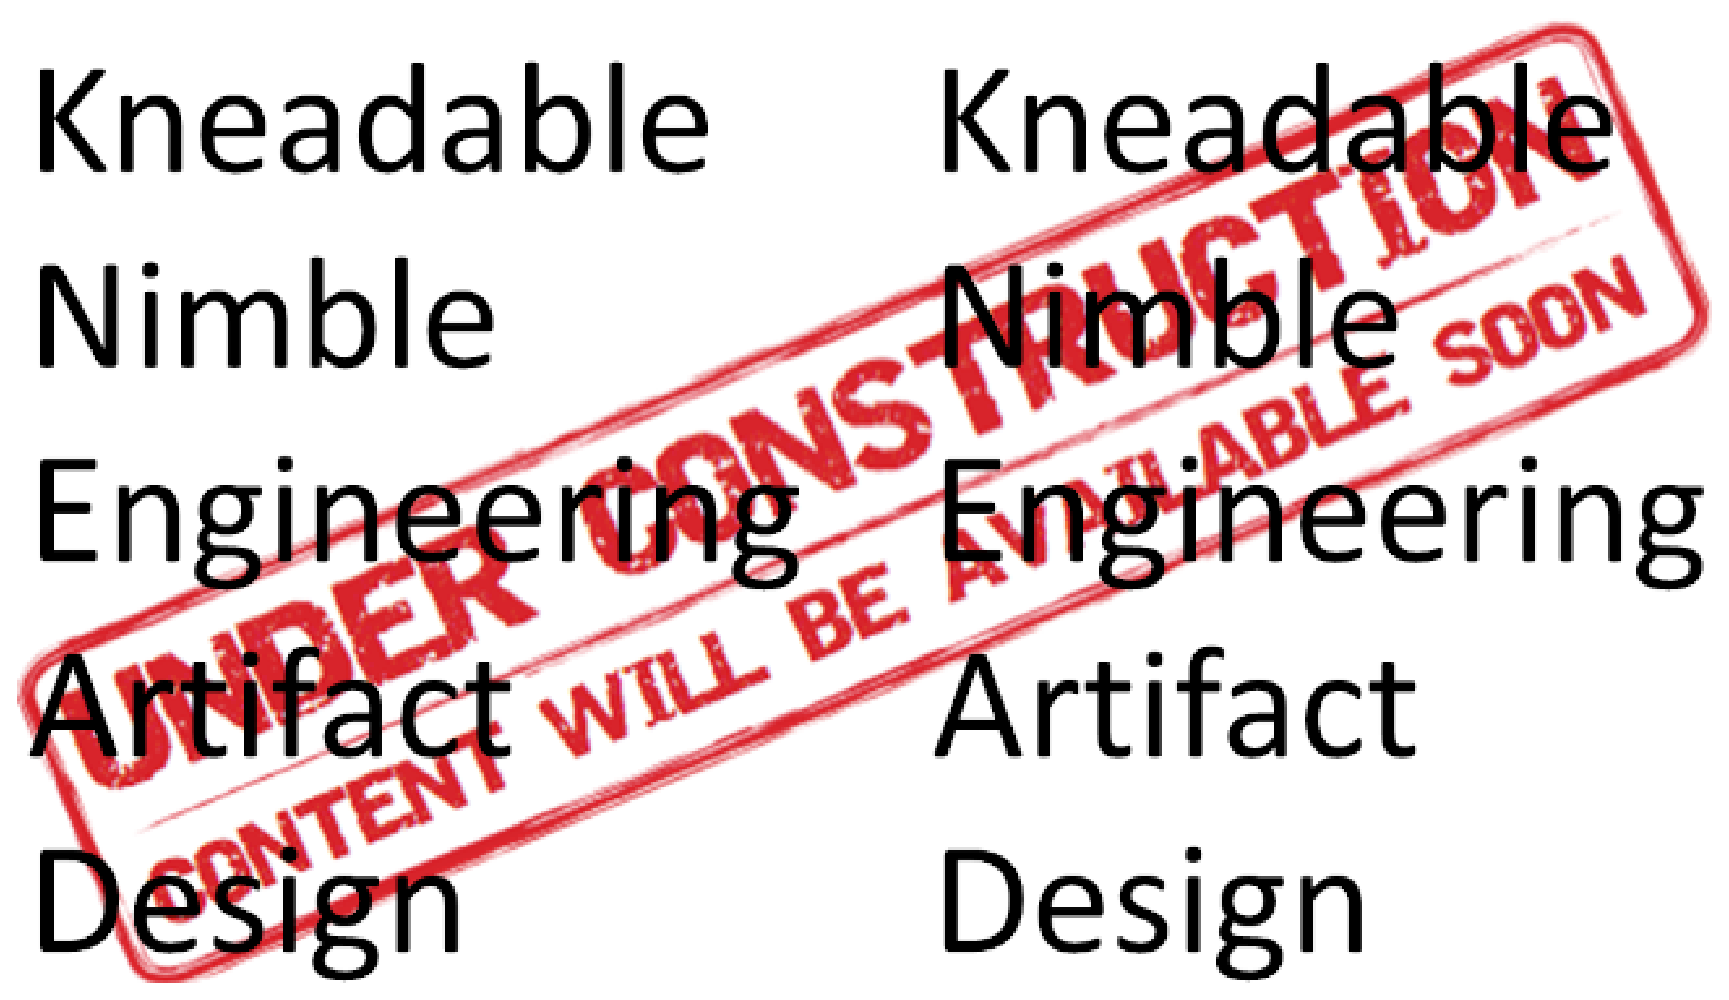
\includegraphics[width=6in]{../zProjectWideData/images/KNEAD_UnderConstruction_100dpi_6.5inchesWide.eps}
		\fi
		\caption{System Overview}
	\label{fig:SystemOverview}
\end{figure}
This diagram shows the major external interfaces that provide the capabilities of \ThisSys.
As are shown, the \ThisSys can provide \TBD.

This system would be a game where the user would have to balance a ball on a LCD screen that is builtin on the STM32 board. We shall read data from an MEM every single frame.
\ThisSys would keep track of the current position of the ball and where the next updated move is. This helps keep track of the system of where the ball is until a movment occure.
\ThisSys shall process at a maximum 180 Hz. This would give the user enough time to process the current angle of the ball and be able to present on the LCD-TFT screen.